\documentclass[twoside]{book}

% Packages required by doxygen
\usepackage{calc}
\usepackage{doxygen}
\usepackage{graphicx}
\usepackage[utf8]{inputenc}
\usepackage{makeidx}
\usepackage{multicol}
\usepackage{multirow}
\usepackage{textcomp}
\usepackage[table]{xcolor}

% Font selection
\usepackage[T1]{fontenc}
\usepackage{mathptmx}
\usepackage[scaled=.90]{helvet}
\usepackage{courier}
\usepackage{amssymb}
\usepackage{sectsty}
\renewcommand{\familydefault}{\sfdefault}
\allsectionsfont{%
  \fontseries{bc}\selectfont%
  \color{darkgray}%
}
\renewcommand{\DoxyLabelFont}{%
  \fontseries{bc}\selectfont%
  \color{darkgray}%
}

% Page & text layout
\usepackage{geometry}
\geometry{%
  a4paper,%
  top=2.5cm,%
  bottom=2.5cm,%
  left=2.5cm,%
  right=2.5cm%
}
\tolerance=750
\hfuzz=15pt
\hbadness=750
\setlength{\emergencystretch}{15pt}
\setlength{\parindent}{0cm}
\setlength{\parskip}{0.2cm}
\makeatletter
\renewcommand{\paragraph}{%
  \@startsection{paragraph}{4}{0ex}{-1.0ex}{1.0ex}{%
    \normalfont\normalsize\bfseries\SS@parafont%
  }%
}
\renewcommand{\subparagraph}{%
  \@startsection{subparagraph}{5}{0ex}{-1.0ex}{1.0ex}{%
    \normalfont\normalsize\bfseries\SS@subparafont%
  }%
}
\makeatother

% Headers & footers
\usepackage{fancyhdr}
\pagestyle{fancyplain}
\fancyhead[LE]{\fancyplain{}{\bfseries\thepage}}
\fancyhead[CE]{\fancyplain{}{}}
\fancyhead[RE]{\fancyplain{}{\bfseries\leftmark}}
\fancyhead[LO]{\fancyplain{}{\bfseries\rightmark}}
\fancyhead[CO]{\fancyplain{}{}}
\fancyhead[RO]{\fancyplain{}{\bfseries\thepage}}
\fancyfoot[LE]{\fancyplain{}{}}
\fancyfoot[CE]{\fancyplain{}{}}
\fancyfoot[RE]{\fancyplain{}{\bfseries\scriptsize Generated on Thu Apr 16 2015 10\-:34\-:19 for My Project by Doxygen }}
\fancyfoot[LO]{\fancyplain{}{\bfseries\scriptsize Generated on Thu Apr 16 2015 10\-:34\-:19 for My Project by Doxygen }}
\fancyfoot[CO]{\fancyplain{}{}}
\fancyfoot[RO]{\fancyplain{}{}}
\renewcommand{\footrulewidth}{0.4pt}
\renewcommand{\chaptermark}[1]{%
  \markboth{#1}{}%
}
\renewcommand{\sectionmark}[1]{%
  \markright{\thesection\ #1}%
}

% Indices & bibliography
\usepackage{natbib}
\usepackage[titles]{tocloft}
\setcounter{tocdepth}{3}
\setcounter{secnumdepth}{5}
\makeindex

% Hyperlinks (required, but should be loaded last)
\usepackage{ifpdf}
\ifpdf
  \usepackage[pdftex,pagebackref=true]{hyperref}
\else
  \usepackage[ps2pdf,pagebackref=true]{hyperref}
\fi
\hypersetup{%
  colorlinks=true,%
  linkcolor=blue,%
  citecolor=blue,%
  unicode%
}

% Custom commands
\newcommand{\clearemptydoublepage}{%
  \newpage{\pagestyle{empty}\cleardoublepage}%
}


%===== C O N T E N T S =====

\begin{document}

% Titlepage & ToC
\hypersetup{pageanchor=false}
\pagenumbering{roman}
\begin{titlepage}
\vspace*{7cm}
\begin{center}%
{\Large My Project }\\
\vspace*{1cm}
{\large Generated by Doxygen 1.8.6}\\
\vspace*{0.5cm}
{\small Thu Apr 16 2015 10:34:19}\\
\end{center}
\end{titlepage}
\clearemptydoublepage
\tableofcontents
\clearemptydoublepage
\pagenumbering{arabic}
\hypersetup{pageanchor=true}

%--- Begin generated contents ---
\chapter{Hierarchical Index}
\section{Class Hierarchy}
This inheritance list is sorted roughly, but not completely, alphabetically\-:\begin{DoxyCompactList}
\item \contentsline{section}{csis3700\-:\-:collision}{\pageref{classcsis3700_1_1collision}}{}
\item \contentsline{section}{csis3700\-:\-:image\-\_\-library}{\pageref{classcsis3700_1_1image__library}}{}
\item \contentsline{section}{csis3700\-:\-:image\-\_\-sequence}{\pageref{classcsis3700_1_1image__sequence}}{}
\item \contentsline{section}{csis3700\-:\-:image\-\_\-with\-\_\-offset}{\pageref{classcsis3700_1_1image__with__offset}}{}
\item \contentsline{section}{csis3700\-:\-:keyboard\-\_\-manager}{\pageref{classcsis3700_1_1keyboard__manager}}{}
\item \contentsline{section}{csis3700\-:\-:rectangle}{\pageref{classcsis3700_1_1rectangle}}{}
\item \contentsline{section}{csis3700\-:\-:sprite}{\pageref{classcsis3700_1_1sprite}}{}
\begin{DoxyCompactList}
\item \contentsline{section}{csis3700\-:\-:obstruction\-\_\-sprite}{\pageref{classcsis3700_1_1obstruction__sprite}}{}
\item \contentsline{section}{csis3700\-:\-:phys\-\_\-sprite}{\pageref{classcsis3700_1_1phys__sprite}}{}
\begin{DoxyCompactList}
\item \contentsline{section}{csis3700\-:\-:player\-\_\-sprite}{\pageref{classcsis3700_1_1player__sprite}}{}
\end{DoxyCompactList}
\end{DoxyCompactList}
\item \contentsline{section}{csis3700\-:\-:vec2d}{\pageref{classcsis3700_1_1vec2d}}{}
\item \contentsline{section}{csis3700\-:\-:world}{\pageref{classcsis3700_1_1world}}{}
\end{DoxyCompactList}

\chapter{Class Index}
\section{Class List}
Here are the classes, structs, unions and interfaces with brief descriptions\-:\begin{DoxyCompactList}
\item\contentsline{section}{\hyperlink{classcsis3700_1_1collision}{csis3700\-::collision} }{\pageref{classcsis3700_1_1collision}}{}
\item\contentsline{section}{\hyperlink{classcsis3700_1_1image__library}{csis3700\-::image\-\_\-library} }{\pageref{classcsis3700_1_1image__library}}{}
\item\contentsline{section}{\hyperlink{classcsis3700_1_1image__sequence}{csis3700\-::image\-\_\-sequence} }{\pageref{classcsis3700_1_1image__sequence}}{}
\item\contentsline{section}{\hyperlink{classcsis3700_1_1image__with__offset}{csis3700\-::image\-\_\-with\-\_\-offset} }{\pageref{classcsis3700_1_1image__with__offset}}{}
\item\contentsline{section}{\hyperlink{classcsis3700_1_1keyboard__manager}{csis3700\-::keyboard\-\_\-manager} }{\pageref{classcsis3700_1_1keyboard__manager}}{}
\item\contentsline{section}{\hyperlink{classcsis3700_1_1obstruction__sprite}{csis3700\-::obstruction\-\_\-sprite} }{\pageref{classcsis3700_1_1obstruction__sprite}}{}
\item\contentsline{section}{\hyperlink{classcsis3700_1_1phys__sprite}{csis3700\-::phys\-\_\-sprite} }{\pageref{classcsis3700_1_1phys__sprite}}{}
\item\contentsline{section}{\hyperlink{classcsis3700_1_1player__sprite}{csis3700\-::player\-\_\-sprite} }{\pageref{classcsis3700_1_1player__sprite}}{}
\item\contentsline{section}{\hyperlink{classcsis3700_1_1rectangle}{csis3700\-::rectangle} }{\pageref{classcsis3700_1_1rectangle}}{}
\item\contentsline{section}{\hyperlink{classcsis3700_1_1sprite}{csis3700\-::sprite} }{\pageref{classcsis3700_1_1sprite}}{}
\item\contentsline{section}{\hyperlink{classcsis3700_1_1vec2d}{csis3700\-::vec2d} }{\pageref{classcsis3700_1_1vec2d}}{}
\item\contentsline{section}{\hyperlink{classcsis3700_1_1world}{csis3700\-::world} }{\pageref{classcsis3700_1_1world}}{}
\end{DoxyCompactList}

\chapter{Class Documentation}
\hypertarget{classcsis3700_1_1collision}{\section{csis3700\-:\-:collision Class Reference}
\label{classcsis3700_1_1collision}\index{csis3700\-::collision@{csis3700\-::collision}}
}
\subsection*{Public Member Functions}
\begin{DoxyCompactItemize}
\item 
\hypertarget{classcsis3700_1_1collision_a28ce4cf4d73a43840adaf882a7f680da}{{\bfseries collision} (\hyperlink{classcsis3700_1_1sprite}{sprite} $\ast$p1, \hyperlink{classcsis3700_1_1sprite}{sprite} $\ast$p2)}\label{classcsis3700_1_1collision_a28ce4cf4d73a43840adaf882a7f680da}

\item 
\hypertarget{classcsis3700_1_1collision_a5a0054399a8f03e0ad9b10c70ced45c0}{void {\bfseries resolve} ()}\label{classcsis3700_1_1collision_a5a0054399a8f03e0ad9b10c70ced45c0}

\item 
\hypertarget{classcsis3700_1_1collision_ab3e4b0edb6c96d2ea25e0c7eddcae79e}{bool {\bfseries is\-\_\-active} () const }\label{classcsis3700_1_1collision_ab3e4b0edb6c96d2ea25e0c7eddcae79e}

\item 
\hypertarget{classcsis3700_1_1collision_afa074671651c61167ebac3f13a629931}{\hyperlink{classcsis3700_1_1rectangle}{rectangle} {\bfseries collision\-\_\-rectangle} () const }\label{classcsis3700_1_1collision_afa074671651c61167ebac3f13a629931}

\item 
\hypertarget{classcsis3700_1_1collision_a5d82964543afa431f20467978e8c24bc}{bool {\bfseries operator$<$} (const \hyperlink{classcsis3700_1_1collision}{collision} \&other) const }\label{classcsis3700_1_1collision_a5d82964543afa431f20467978e8c24bc}

\end{DoxyCompactItemize}


The documentation for this class was generated from the following files\-:\begin{DoxyCompactItemize}
\item 
collision.\-h\item 
collision.\-C\end{DoxyCompactItemize}

\hypertarget{classcsis3700_1_1image__library}{\section{csis3700\-:\-:image\-\_\-library Class Reference}
\label{classcsis3700_1_1image__library}\index{csis3700\-::image\-\_\-library@{csis3700\-::image\-\_\-library}}
}
\subsection*{Public Member Functions}
\begin{DoxyCompactItemize}
\item 
\hypertarget{classcsis3700_1_1image__library_adea94b7de53bcbedb0612286285521e0}{{\bfseries image\-\_\-library} (std\-::string dir)}\label{classcsis3700_1_1image__library_adea94b7de53bcbedb0612286285521e0}

\item 
\hypertarget{classcsis3700_1_1image__library_a40e4bc8bf2b83ef1e86acef16943ddf5}{A\-L\-L\-E\-G\-R\-O\-\_\-\-B\-I\-T\-M\-A\-P $\ast$ {\bfseries get} (std\-::string name)}\label{classcsis3700_1_1image__library_a40e4bc8bf2b83ef1e86acef16943ddf5}

\end{DoxyCompactItemize}
\subsection*{Static Public Member Functions}
\begin{DoxyCompactItemize}
\item 
static \hyperlink{classcsis3700_1_1image__library}{image\-\_\-library} $\ast$ \hyperlink{classcsis3700_1_1image__library_a0c716935a287fd510951cda2b490f396}{get\-\_\-instance} ()
\end{DoxyCompactItemize}


\subsection{Member Function Documentation}
\hypertarget{classcsis3700_1_1image__library_a0c716935a287fd510951cda2b490f396}{\index{csis3700\-::image\-\_\-library@{csis3700\-::image\-\_\-library}!get\-\_\-instance@{get\-\_\-instance}}
\index{get\-\_\-instance@{get\-\_\-instance}!csis3700::image_library@{csis3700\-::image\-\_\-library}}
\subsubsection[{get\-\_\-instance}]{\setlength{\rightskip}{0pt plus 5cm}{\bf image\-\_\-library} $\ast$ csis3700\-::image\-\_\-library\-::get\-\_\-instance (
\begin{DoxyParamCaption}
{}
\end{DoxyParamCaption}
)\hspace{0.3cm}{\ttfamily [static]}}}\label{classcsis3700_1_1image__library_a0c716935a287fd510951cda2b490f396}
There should only be one instance of \hyperlink{classcsis3700_1_1image__library}{image\-\_\-library} in your application. Use this method to fetch that library. You call it with \hyperlink{classcsis3700_1_1image__library_a0c716935a287fd510951cda2b490f396}{image\-\_\-library\-::get\-\_\-instance()}. 

The documentation for this class was generated from the following files\-:\begin{DoxyCompactItemize}
\item 
image\-\_\-library.\-h\item 
image\-\_\-library.\-C\end{DoxyCompactItemize}

\hypertarget{classcsis3700_1_1image__sequence}{\section{csis3700\-:\-:image\-\_\-sequence Class Reference}
\label{classcsis3700_1_1image__sequence}\index{csis3700\-::image\-\_\-sequence@{csis3700\-::image\-\_\-sequence}}
}
\subsection*{Public Member Functions}
\begin{DoxyCompactItemize}
\item 
void \hyperlink{classcsis3700_1_1image__sequence_aa8c137829b803075fccc0d2549b0df95}{add\-\_\-image} (A\-L\-L\-E\-G\-R\-O\-\_\-\-B\-I\-T\-M\-A\-P $\ast$image, double offset)
\item 
void \hyperlink{classcsis3700_1_1image__sequence_a4a7dadd01b965db2052439584171f7a6}{draw} (double time, float x, float y)
\item 
void \hyperlink{classcsis3700_1_1image__sequence_aa1a83d01babd833a16ac89759a4e0a57}{set\-\_\-loop\-\_\-index} (std\-::size\-\_\-t loop\-\_\-index)
\item 
int \hyperlink{classcsis3700_1_1image__sequence_adbd7345e70b84e0712c980fc862040c5}{get\-\_\-width} () const 
\item 
int \hyperlink{classcsis3700_1_1image__sequence_ad29fb3a6705095bc92223ff565bbc1cf}{get\-\_\-height} () const 
\end{DoxyCompactItemize}


\subsection{Member Function Documentation}
\hypertarget{classcsis3700_1_1image__sequence_aa8c137829b803075fccc0d2549b0df95}{\index{csis3700\-::image\-\_\-sequence@{csis3700\-::image\-\_\-sequence}!add\-\_\-image@{add\-\_\-image}}
\index{add\-\_\-image@{add\-\_\-image}!csis3700::image_sequence@{csis3700\-::image\-\_\-sequence}}
\subsubsection[{add\-\_\-image}]{\setlength{\rightskip}{0pt plus 5cm}void csis3700\-::image\-\_\-sequence\-::add\-\_\-image (
\begin{DoxyParamCaption}
\item[{A\-L\-L\-E\-G\-R\-O\-\_\-\-B\-I\-T\-M\-A\-P $\ast$}]{image, }
\item[{double}]{offset}
\end{DoxyParamCaption}
)}}\label{classcsis3700_1_1image__sequence_aa8c137829b803075fccc0d2549b0df95}
Adds an image to this sequence which will play offset seconds from the previous image. \hypertarget{classcsis3700_1_1image__sequence_a4a7dadd01b965db2052439584171f7a6}{\index{csis3700\-::image\-\_\-sequence@{csis3700\-::image\-\_\-sequence}!draw@{draw}}
\index{draw@{draw}!csis3700::image_sequence@{csis3700\-::image\-\_\-sequence}}
\subsubsection[{draw}]{\setlength{\rightskip}{0pt plus 5cm}void csis3700\-::image\-\_\-sequence\-::draw (
\begin{DoxyParamCaption}
\item[{double}]{time, }
\item[{float}]{x, }
\item[{float}]{y}
\end{DoxyParamCaption}
)}}\label{classcsis3700_1_1image__sequence_a4a7dadd01b965db2052439584171f7a6}
Draw the current image on the current allegro target. \hypertarget{classcsis3700_1_1image__sequence_ad29fb3a6705095bc92223ff565bbc1cf}{\index{csis3700\-::image\-\_\-sequence@{csis3700\-::image\-\_\-sequence}!get\-\_\-height@{get\-\_\-height}}
\index{get\-\_\-height@{get\-\_\-height}!csis3700::image_sequence@{csis3700\-::image\-\_\-sequence}}
\subsubsection[{get\-\_\-height}]{\setlength{\rightskip}{0pt plus 5cm}int csis3700\-::image\-\_\-sequence\-::get\-\_\-height (
\begin{DoxyParamCaption}
{}
\end{DoxyParamCaption}
) const}}\label{classcsis3700_1_1image__sequence_ad29fb3a6705095bc92223ff565bbc1cf}
Returns the height of the first image in the sequence \hypertarget{classcsis3700_1_1image__sequence_adbd7345e70b84e0712c980fc862040c5}{\index{csis3700\-::image\-\_\-sequence@{csis3700\-::image\-\_\-sequence}!get\-\_\-width@{get\-\_\-width}}
\index{get\-\_\-width@{get\-\_\-width}!csis3700::image_sequence@{csis3700\-::image\-\_\-sequence}}
\subsubsection[{get\-\_\-width}]{\setlength{\rightskip}{0pt plus 5cm}int csis3700\-::image\-\_\-sequence\-::get\-\_\-width (
\begin{DoxyParamCaption}
{}
\end{DoxyParamCaption}
) const}}\label{classcsis3700_1_1image__sequence_adbd7345e70b84e0712c980fc862040c5}
Returns the width of the first image in the sequence \hypertarget{classcsis3700_1_1image__sequence_aa1a83d01babd833a16ac89759a4e0a57}{\index{csis3700\-::image\-\_\-sequence@{csis3700\-::image\-\_\-sequence}!set\-\_\-loop\-\_\-index@{set\-\_\-loop\-\_\-index}}
\index{set\-\_\-loop\-\_\-index@{set\-\_\-loop\-\_\-index}!csis3700::image_sequence@{csis3700\-::image\-\_\-sequence}}
\subsubsection[{set\-\_\-loop\-\_\-index}]{\setlength{\rightskip}{0pt plus 5cm}void csis3700\-::image\-\_\-sequence\-::set\-\_\-loop\-\_\-index (
\begin{DoxyParamCaption}
\item[{std\-::size\-\_\-t}]{loop\-\_\-index}
\end{DoxyParamCaption}
)}}\label{classcsis3700_1_1image__sequence_aa1a83d01babd833a16ac89759a4e0a57}
Set the loop index. When the last image in the sequence is reached, the image at this index will be next. Defaults to 0 (zero). 

The documentation for this class was generated from the following files\-:\begin{DoxyCompactItemize}
\item 
image\-\_\-sequence.\-h\item 
image\-\_\-sequence.\-C\end{DoxyCompactItemize}

\hypertarget{classcsis3700_1_1image__with__offset}{\section{csis3700\-:\-:image\-\_\-with\-\_\-offset Class Reference}
\label{classcsis3700_1_1image__with__offset}\index{csis3700\-::image\-\_\-with\-\_\-offset@{csis3700\-::image\-\_\-with\-\_\-offset}}
}
\subsection*{Public Member Functions}
\begin{DoxyCompactItemize}
\item 
\hypertarget{classcsis3700_1_1image__with__offset_ad9d01a0d16d8f36981054d6f16967d1f}{{\bfseries image\-\_\-with\-\_\-offset} (A\-L\-L\-E\-G\-R\-O\-\_\-\-B\-I\-T\-M\-A\-P $\ast$image, double offset)}\label{classcsis3700_1_1image__with__offset_ad9d01a0d16d8f36981054d6f16967d1f}

\end{DoxyCompactItemize}
\subsection*{Public Attributes}
\begin{DoxyCompactItemize}
\item 
\hypertarget{classcsis3700_1_1image__with__offset_a9440b6eb66dfad9a7bf83b5dfe8baf86}{A\-L\-L\-E\-G\-R\-O\-\_\-\-B\-I\-T\-M\-A\-P $\ast$ {\bfseries image}}\label{classcsis3700_1_1image__with__offset_a9440b6eb66dfad9a7bf83b5dfe8baf86}

\item 
\hypertarget{classcsis3700_1_1image__with__offset_a15708b2a95ca7a765baccb19df7bd0c6}{double {\bfseries offset}}\label{classcsis3700_1_1image__with__offset_a15708b2a95ca7a765baccb19df7bd0c6}

\end{DoxyCompactItemize}


The documentation for this class was generated from the following files\-:\begin{DoxyCompactItemize}
\item 
image\-\_\-sequence.\-h\item 
image\-\_\-sequence.\-C\end{DoxyCompactItemize}

\hypertarget{classcsis3700_1_1keyboard__manager}{\section{csis3700\-:\-:keyboard\-\_\-manager Class Reference}
\label{classcsis3700_1_1keyboard__manager}\index{csis3700\-::keyboard\-\_\-manager@{csis3700\-::keyboard\-\_\-manager}}
}
\subsection*{Public Member Functions}
\begin{DoxyCompactItemize}
\item 
bool \hyperlink{classcsis3700_1_1keyboard__manager_a6171a0c3677e5e08ddff2bf48b65755d}{is\-\_\-key\-\_\-down} (int keycode)
\item 
void \hyperlink{classcsis3700_1_1keyboard__manager_aae677b5185c2d235b589767c4e3e6098}{key\-\_\-down} (int keycode)
\item 
void \hyperlink{classcsis3700_1_1keyboard__manager_a970b26d49eb327f582ac28ac6caa0f36}{key\-\_\-up} (int keycode)
\end{DoxyCompactItemize}
\subsection*{Static Public Member Functions}
\begin{DoxyCompactItemize}
\item 
\hypertarget{classcsis3700_1_1keyboard__manager_afcaf721946fca027c9525e539691d58a}{static \hyperlink{classcsis3700_1_1keyboard__manager}{keyboard\-\_\-manager} $\ast$ {\bfseries get\-\_\-instance} ()}\label{classcsis3700_1_1keyboard__manager_afcaf721946fca027c9525e539691d58a}

\end{DoxyCompactItemize}


\subsection{Member Function Documentation}
\hypertarget{classcsis3700_1_1keyboard__manager_a6171a0c3677e5e08ddff2bf48b65755d}{\index{csis3700\-::keyboard\-\_\-manager@{csis3700\-::keyboard\-\_\-manager}!is\-\_\-key\-\_\-down@{is\-\_\-key\-\_\-down}}
\index{is\-\_\-key\-\_\-down@{is\-\_\-key\-\_\-down}!csis3700::keyboard_manager@{csis3700\-::keyboard\-\_\-manager}}
\subsubsection[{is\-\_\-key\-\_\-down}]{\setlength{\rightskip}{0pt plus 5cm}bool csis3700\-::keyboard\-\_\-manager\-::is\-\_\-key\-\_\-down (
\begin{DoxyParamCaption}
\item[{int}]{keycode}
\end{DoxyParamCaption}
)}}\label{classcsis3700_1_1keyboard__manager_a6171a0c3677e5e08ddff2bf48b65755d}
Answers true iff the specified key currently held down \hypertarget{classcsis3700_1_1keyboard__manager_aae677b5185c2d235b589767c4e3e6098}{\index{csis3700\-::keyboard\-\_\-manager@{csis3700\-::keyboard\-\_\-manager}!key\-\_\-down@{key\-\_\-down}}
\index{key\-\_\-down@{key\-\_\-down}!csis3700::keyboard_manager@{csis3700\-::keyboard\-\_\-manager}}
\subsubsection[{key\-\_\-down}]{\setlength{\rightskip}{0pt plus 5cm}void csis3700\-::keyboard\-\_\-manager\-::key\-\_\-down (
\begin{DoxyParamCaption}
\item[{int}]{keycode}
\end{DoxyParamCaption}
)}}\label{classcsis3700_1_1keyboard__manager_aae677b5185c2d235b589767c4e3e6098}
Called when a key is pressed \hypertarget{classcsis3700_1_1keyboard__manager_a970b26d49eb327f582ac28ac6caa0f36}{\index{csis3700\-::keyboard\-\_\-manager@{csis3700\-::keyboard\-\_\-manager}!key\-\_\-up@{key\-\_\-up}}
\index{key\-\_\-up@{key\-\_\-up}!csis3700::keyboard_manager@{csis3700\-::keyboard\-\_\-manager}}
\subsubsection[{key\-\_\-up}]{\setlength{\rightskip}{0pt plus 5cm}void csis3700\-::keyboard\-\_\-manager\-::key\-\_\-up (
\begin{DoxyParamCaption}
\item[{int}]{keycode}
\end{DoxyParamCaption}
)}}\label{classcsis3700_1_1keyboard__manager_a970b26d49eb327f582ac28ac6caa0f36}
Called when a key is released 

The documentation for this class was generated from the following files\-:\begin{DoxyCompactItemize}
\item 
keyboard\-\_\-manager.\-h\item 
keyboard\-\_\-manager.\-C\end{DoxyCompactItemize}

\hypertarget{classcsis3700_1_1obstruction__sprite}{\section{csis3700\-:\-:obstruction\-\_\-sprite Class Reference}
\label{classcsis3700_1_1obstruction__sprite}\index{csis3700\-::obstruction\-\_\-sprite@{csis3700\-::obstruction\-\_\-sprite}}
}


{\ttfamily \#include $<$obstruction\-\_\-sprite.\-h$>$}

Inheritance diagram for csis3700\-:\-:obstruction\-\_\-sprite\-:\begin{figure}[H]
\begin{center}
\leavevmode
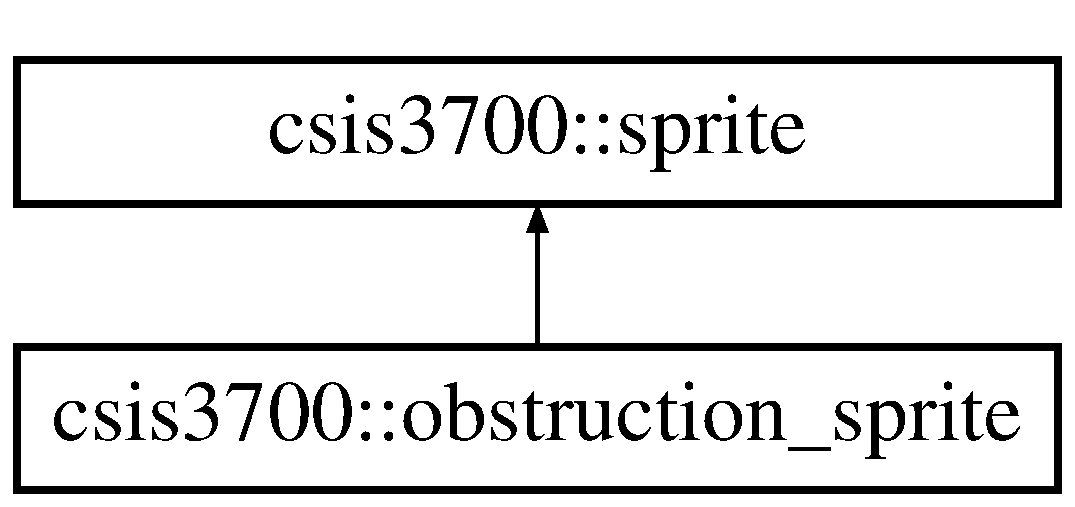
\includegraphics[height=2.000000cm]{classcsis3700_1_1obstruction__sprite}
\end{center}
\end{figure}
\subsection*{Public Member Functions}
\begin{DoxyCompactItemize}
\item 
\hypertarget{classcsis3700_1_1obstruction__sprite_a9d7f66afeeb3dba404c602b54eeb3308}{{\bfseries obstruction\-\_\-sprite} (float initial\-\_\-x, float initial\-\_\-y, A\-L\-L\-E\-G\-R\-O\-\_\-\-B\-I\-T\-M\-A\-P $\ast$image=N\-U\-L\-L)}\label{classcsis3700_1_1obstruction__sprite_a9d7f66afeeb3dba404c602b54eeb3308}

\item 
\hypertarget{classcsis3700_1_1obstruction__sprite_a6629cd0d13f54ed8666326ca55fb7c0c}{virtual void {\bfseries set\-\_\-velocity} (const \hyperlink{classcsis3700_1_1vec2d}{vec2d} \&v)}\label{classcsis3700_1_1obstruction__sprite_a6629cd0d13f54ed8666326ca55fb7c0c}

\item 
\hypertarget{classcsis3700_1_1obstruction__sprite_a4b2102c43b49b91b4186f074ebbcc886}{virtual \hyperlink{classcsis3700_1_1vec2d}{vec2d} {\bfseries get\-\_\-velocity} () const }\label{classcsis3700_1_1obstruction__sprite_a4b2102c43b49b91b4186f074ebbcc886}

\item 
\hypertarget{classcsis3700_1_1obstruction__sprite_a1ce0b8681cfb6020a332cd97843b4a88}{virtual void {\bfseries resolve} (const \hyperlink{classcsis3700_1_1collision}{collision} \&\hyperlink{classcsis3700_1_1collision}{collision}, \hyperlink{classcsis3700_1_1sprite}{sprite} $\ast$other)}\label{classcsis3700_1_1obstruction__sprite_a1ce0b8681cfb6020a332cd97843b4a88}

\end{DoxyCompactItemize}
\subsection*{Additional Inherited Members}


\subsection{Detailed Description}
obstruction\-\_\-sprites don't typically move and when they participate in a collision they are unimpacted by it. They typically render themslves as a single, static bitmap. 

The documentation for this class was generated from the following files\-:\begin{DoxyCompactItemize}
\item 
obstruction\-\_\-sprite.\-h\item 
obstruction\-\_\-sprite.\-C\end{DoxyCompactItemize}

\hypertarget{classcsis3700_1_1phys__sprite}{\section{csis3700\-:\-:phys\-\_\-sprite Class Reference}
\label{classcsis3700_1_1phys__sprite}\index{csis3700\-::phys\-\_\-sprite@{csis3700\-::phys\-\_\-sprite}}
}


{\ttfamily \#include $<$phys\-\_\-sprite.\-h$>$}

Inheritance diagram for csis3700\-:\-:phys\-\_\-sprite\-:\begin{figure}[H]
\begin{center}
\leavevmode
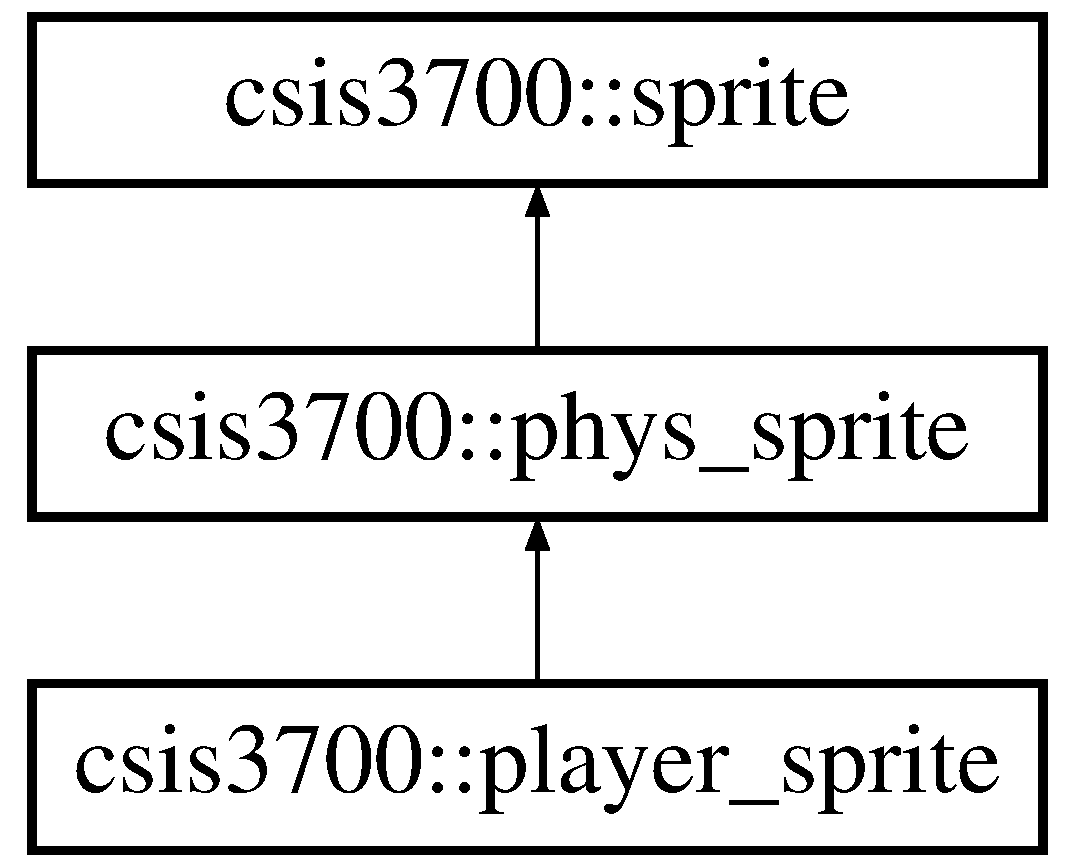
\includegraphics[height=3.000000cm]{classcsis3700_1_1phys__sprite}
\end{center}
\end{figure}
\subsection*{Public Member Functions}
\begin{DoxyCompactItemize}
\item 
\hypertarget{classcsis3700_1_1phys__sprite_a300b8fcf6d18176c9dced92cd90edd99}{{\bfseries phys\-\_\-sprite} (float initial\-\_\-x=0, float initial\-\_\-y=0, float initial\-\_\-vx=0, float initial\-\_\-vy=0)}\label{classcsis3700_1_1phys__sprite_a300b8fcf6d18176c9dced92cd90edd99}

\item 
virtual void \hyperlink{classcsis3700_1_1phys__sprite_a3bb24599b1bc2fd13846826308914db4}{advance\-\_\-by\-\_\-time} (double dt)
\item 
\hypertarget{classcsis3700_1_1phys__sprite_af69d2201b23b3ebc3e81757f473285a1}{virtual \hyperlink{classcsis3700_1_1vec2d}{vec2d} {\bfseries get\-\_\-acceleration} () const }\label{classcsis3700_1_1phys__sprite_af69d2201b23b3ebc3e81757f473285a1}

\item 
\hypertarget{classcsis3700_1_1phys__sprite_a72682ff328159518f110a935ff8670dd}{virtual \hyperlink{classcsis3700_1_1vec2d}{vec2d} {\bfseries get\-\_\-velocity} () const }\label{classcsis3700_1_1phys__sprite_a72682ff328159518f110a935ff8670dd}

\item 
\hypertarget{classcsis3700_1_1phys__sprite_a2dd7b26fd33125f84f3eccabac146dcd}{virtual void {\bfseries set\-\_\-velocity} (const \hyperlink{classcsis3700_1_1vec2d}{vec2d} \&v)}\label{classcsis3700_1_1phys__sprite_a2dd7b26fd33125f84f3eccabac146dcd}

\item 
\hypertarget{classcsis3700_1_1phys__sprite_ade2d0f1d3e03981d89a8549ec3a1999c}{virtual void {\bfseries add\-\_\-force} (\hyperlink{classcsis3700_1_1vec2d}{vec2d} f)}\label{classcsis3700_1_1phys__sprite_ade2d0f1d3e03981d89a8549ec3a1999c}

\end{DoxyCompactItemize}
\subsection*{Additional Inherited Members}


\subsection{Detailed Description}
Physical sprites move using an approximation of newtonian kinematics. 

\subsection{Member Function Documentation}
\hypertarget{classcsis3700_1_1phys__sprite_a3bb24599b1bc2fd13846826308914db4}{\index{csis3700\-::phys\-\_\-sprite@{csis3700\-::phys\-\_\-sprite}!advance\-\_\-by\-\_\-time@{advance\-\_\-by\-\_\-time}}
\index{advance\-\_\-by\-\_\-time@{advance\-\_\-by\-\_\-time}!csis3700::phys_sprite@{csis3700\-::phys\-\_\-sprite}}
\subsubsection[{advance\-\_\-by\-\_\-time}]{\setlength{\rightskip}{0pt plus 5cm}void csis3700\-::phys\-\_\-sprite\-::advance\-\_\-by\-\_\-time (
\begin{DoxyParamCaption}
\item[{double}]{dt}
\end{DoxyParamCaption}
)\hspace{0.3cm}{\ttfamily [virtual]}}}\label{classcsis3700_1_1phys__sprite_a3bb24599b1bc2fd13846826308914db4}
Move time forward by the specified amount 

Reimplemented from \hyperlink{classcsis3700_1_1sprite_ac4d932bda87ce98a36579de3e1392a8f}{csis3700\-::sprite}.



Reimplemented in \hyperlink{classcsis3700_1_1player__sprite_ac2453e0b3934ac639d704c4ecca7493d}{csis3700\-::player\-\_\-sprite}.



The documentation for this class was generated from the following files\-:\begin{DoxyCompactItemize}
\item 
phys\-\_\-sprite.\-h\item 
phys\-\_\-sprite.\-C\end{DoxyCompactItemize}

\hypertarget{classcsis3700_1_1player__sprite}{\section{csis3700\-:\-:player\-\_\-sprite Class Reference}
\label{classcsis3700_1_1player__sprite}\index{csis3700\-::player\-\_\-sprite@{csis3700\-::player\-\_\-sprite}}
}
Inheritance diagram for csis3700\-:\-:player\-\_\-sprite\-:\begin{figure}[H]
\begin{center}
\leavevmode
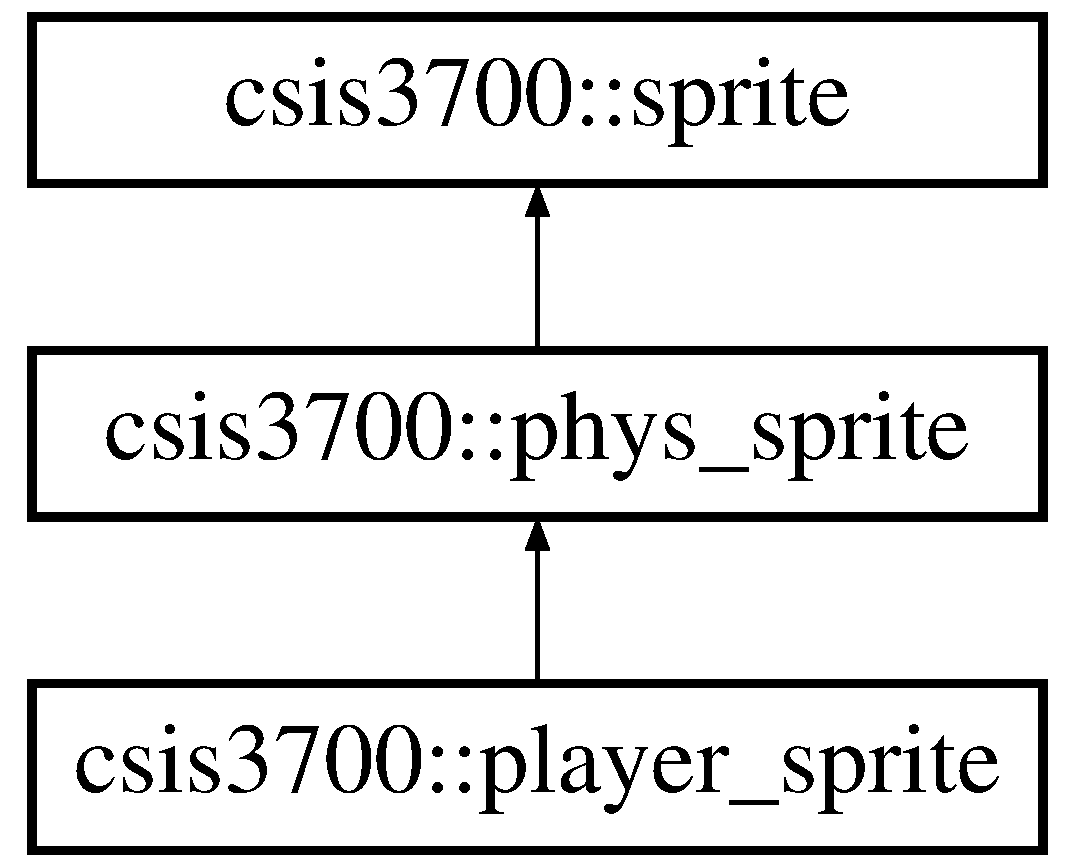
\includegraphics[height=3.000000cm]{classcsis3700_1_1player__sprite}
\end{center}
\end{figure}
\subsection*{Public Member Functions}
\begin{DoxyCompactItemize}
\item 
\hypertarget{classcsis3700_1_1player__sprite_ac187a629d01d5499a19a96e10c132aab}{{\bfseries player\-\_\-sprite} (float initial\-\_\-x=0, float initial\-\_\-y=0)}\label{classcsis3700_1_1player__sprite_ac187a629d01d5499a19a96e10c132aab}

\item 
\hypertarget{classcsis3700_1_1player__sprite_a3c25365425b909f164234f5cd6391ecc}{virtual bool {\bfseries is\-\_\-passive} () const }\label{classcsis3700_1_1player__sprite_a3c25365425b909f164234f5cd6391ecc}

\item 
\hypertarget{classcsis3700_1_1player__sprite_a2fc12d698304e7db48bee063e2cde2be}{virtual void {\bfseries set\-\_\-on\-\_\-ground} (bool v)}\label{classcsis3700_1_1player__sprite_a2fc12d698304e7db48bee063e2cde2be}

\item 
virtual void \hyperlink{classcsis3700_1_1player__sprite_ac2453e0b3934ac639d704c4ecca7493d}{advance\-\_\-by\-\_\-time} (double dt)
\item 
\hypertarget{classcsis3700_1_1player__sprite_a05d3409aa60e9eae24b696c9e9508b7a}{virtual void {\bfseries resolve} (const \hyperlink{classcsis3700_1_1collision}{collision} \&\hyperlink{classcsis3700_1_1collision}{collision}, \hyperlink{classcsis3700_1_1sprite}{sprite} $\ast$other)}\label{classcsis3700_1_1player__sprite_a05d3409aa60e9eae24b696c9e9508b7a}

\end{DoxyCompactItemize}
\subsection*{Additional Inherited Members}


\subsection{Member Function Documentation}
\hypertarget{classcsis3700_1_1player__sprite_ac2453e0b3934ac639d704c4ecca7493d}{\index{csis3700\-::player\-\_\-sprite@{csis3700\-::player\-\_\-sprite}!advance\-\_\-by\-\_\-time@{advance\-\_\-by\-\_\-time}}
\index{advance\-\_\-by\-\_\-time@{advance\-\_\-by\-\_\-time}!csis3700::player_sprite@{csis3700\-::player\-\_\-sprite}}
\subsubsection[{advance\-\_\-by\-\_\-time}]{\setlength{\rightskip}{0pt plus 5cm}void csis3700\-::player\-\_\-sprite\-::advance\-\_\-by\-\_\-time (
\begin{DoxyParamCaption}
\item[{double}]{dt}
\end{DoxyParamCaption}
)\hspace{0.3cm}{\ttfamily [virtual]}}}\label{classcsis3700_1_1player__sprite_ac2453e0b3934ac639d704c4ecca7493d}
Move time forward by the specified amount 

Reimplemented from \hyperlink{classcsis3700_1_1phys__sprite_a3bb24599b1bc2fd13846826308914db4}{csis3700\-::phys\-\_\-sprite}.



The documentation for this class was generated from the following files\-:\begin{DoxyCompactItemize}
\item 
player\-\_\-sprite.\-h\item 
player\-\_\-sprite.\-C\end{DoxyCompactItemize}

\hypertarget{classcsis3700_1_1rectangle}{\section{csis3700\-:\-:rectangle Class Reference}
\label{classcsis3700_1_1rectangle}\index{csis3700\-::rectangle@{csis3700\-::rectangle}}
}


{\ttfamily \#include $<$rectangle.\-h$>$}

\subsection*{Public Member Functions}
\begin{DoxyCompactItemize}
\item 
\hyperlink{classcsis3700_1_1rectangle_a12769987479c35eb82d4c327c5af31fb}{rectangle} (float x, float y, float width, float height)
\item 
\hyperlink{classcsis3700_1_1rectangle_a343355b4f013ac440b155d634ebc1c5c}{rectangle} (\hyperlink{classcsis3700_1_1vec2d}{vec2d} corner, float width, float height)
\item 
\hyperlink{classcsis3700_1_1rectangle_a65e217f0a67f76c2014b34f5995c689d}{rectangle} (\hyperlink{classcsis3700_1_1vec2d}{vec2d} \hyperlink{classcsis3700_1_1rectangle_aab0dc95e90e205d5e4f5e7f636fee8e3}{upper\-\_\-left\-\_\-corner}, \hyperlink{classcsis3700_1_1vec2d}{vec2d} \hyperlink{classcsis3700_1_1rectangle_a5ba599fc8d08e36be15c7d4e017f9d8b}{lower\-\_\-right\-\_\-corner})
\item 
\hypertarget{classcsis3700_1_1rectangle_afcf0790126b736866d883b51bdb5e2c2}{float {\bfseries get\-\_\-width} () const }\label{classcsis3700_1_1rectangle_afcf0790126b736866d883b51bdb5e2c2}

\item 
\hypertarget{classcsis3700_1_1rectangle_ae0826725dc934c151f5ad37b37c9c777}{float {\bfseries get\-\_\-height} () const }\label{classcsis3700_1_1rectangle_ae0826725dc934c151f5ad37b37c9c777}

\item 
\hypertarget{classcsis3700_1_1rectangle_a417cca148168261b1dd6df6f9379c435}{float {\bfseries get\-\_\-area} () const }\label{classcsis3700_1_1rectangle_a417cca148168261b1dd6df6f9379c435}

\item 
\hyperlink{classcsis3700_1_1vec2d}{vec2d} \hyperlink{classcsis3700_1_1rectangle_aab0dc95e90e205d5e4f5e7f636fee8e3}{upper\-\_\-left\-\_\-corner} () const 
\item 
\hyperlink{classcsis3700_1_1vec2d}{vec2d} \hyperlink{classcsis3700_1_1rectangle_a5ba599fc8d08e36be15c7d4e017f9d8b}{lower\-\_\-right\-\_\-corner} () const 
\item 
\hyperlink{classcsis3700_1_1rectangle}{rectangle} \hyperlink{classcsis3700_1_1rectangle_a3f9209f4029bbf57b117d509e041265c}{intersection} (const \hyperlink{classcsis3700_1_1rectangle}{rectangle} \&other) const 
\item 
bool \hyperlink{classcsis3700_1_1rectangle_a1dadf9d8f1f9333a3c5f24e8be295735}{contains} (\hyperlink{classcsis3700_1_1vec2d}{vec2d} point) const 
\item 
bool \hyperlink{classcsis3700_1_1rectangle_ae19050257ed8eb56aab750134798ba7e}{is\-\_\-degenerate} () const 
\end{DoxyCompactItemize}


\subsection{Detailed Description}
I represent an oriented rectangle. My sides are parallel to the x and y axes of the coordinate system. 

\subsection{Constructor \& Destructor Documentation}
\hypertarget{classcsis3700_1_1rectangle_a12769987479c35eb82d4c327c5af31fb}{\index{csis3700\-::rectangle@{csis3700\-::rectangle}!rectangle@{rectangle}}
\index{rectangle@{rectangle}!csis3700::rectangle@{csis3700\-::rectangle}}
\subsubsection[{rectangle}]{\setlength{\rightskip}{0pt plus 5cm}csis3700\-::rectangle\-::rectangle (
\begin{DoxyParamCaption}
\item[{float}]{x, }
\item[{float}]{y, }
\item[{float}]{width, }
\item[{float}]{height}
\end{DoxyParamCaption}
)}}\label{classcsis3700_1_1rectangle_a12769987479c35eb82d4c327c5af31fb}
Construct a rectangle. Note if width or height is negative then this rectangle is considered degenerate (empty). \hypertarget{classcsis3700_1_1rectangle_a343355b4f013ac440b155d634ebc1c5c}{\index{csis3700\-::rectangle@{csis3700\-::rectangle}!rectangle@{rectangle}}
\index{rectangle@{rectangle}!csis3700::rectangle@{csis3700\-::rectangle}}
\subsubsection[{rectangle}]{\setlength{\rightskip}{0pt plus 5cm}csis3700\-::rectangle\-::rectangle (
\begin{DoxyParamCaption}
\item[{{\bf vec2d}}]{corner, }
\item[{float}]{width, }
\item[{float}]{height}
\end{DoxyParamCaption}
)}}\label{classcsis3700_1_1rectangle_a343355b4f013ac440b155d634ebc1c5c}
Construct a rectangle by specifying the position of its upper left corner as well as its dimensions. \hypertarget{classcsis3700_1_1rectangle_a65e217f0a67f76c2014b34f5995c689d}{\index{csis3700\-::rectangle@{csis3700\-::rectangle}!rectangle@{rectangle}}
\index{rectangle@{rectangle}!csis3700::rectangle@{csis3700\-::rectangle}}
\subsubsection[{rectangle}]{\setlength{\rightskip}{0pt plus 5cm}csis3700\-::rectangle\-::rectangle (
\begin{DoxyParamCaption}
\item[{{\bf vec2d}}]{upper\-\_\-left\-\_\-corner, }
\item[{{\bf vec2d}}]{lower\-\_\-right\-\_\-corner}
\end{DoxyParamCaption}
)}}\label{classcsis3700_1_1rectangle_a65e217f0a67f76c2014b34f5995c689d}
Construct a rectangle given two corners. The order of the corners is important. upper\-\_\-left\-\_\-corner must be above and to the left of lower\-\_\-right\-\_\-corner or the rectangle will be degenerate. Note orientation is in terms of typical graphical coordinates (increasing y is down). 

\subsection{Member Function Documentation}
\hypertarget{classcsis3700_1_1rectangle_a1dadf9d8f1f9333a3c5f24e8be295735}{\index{csis3700\-::rectangle@{csis3700\-::rectangle}!contains@{contains}}
\index{contains@{contains}!csis3700::rectangle@{csis3700\-::rectangle}}
\subsubsection[{contains}]{\setlength{\rightskip}{0pt plus 5cm}bool csis3700\-::rectangle\-::contains (
\begin{DoxyParamCaption}
\item[{{\bf vec2d}}]{point}
\end{DoxyParamCaption}
) const}}\label{classcsis3700_1_1rectangle_a1dadf9d8f1f9333a3c5f24e8be295735}
Returns true iff this rectangle contains the point specified by the supplied vector (relative to the origin). \hypertarget{classcsis3700_1_1rectangle_a3f9209f4029bbf57b117d509e041265c}{\index{csis3700\-::rectangle@{csis3700\-::rectangle}!intersection@{intersection}}
\index{intersection@{intersection}!csis3700::rectangle@{csis3700\-::rectangle}}
\subsubsection[{intersection}]{\setlength{\rightskip}{0pt plus 5cm}{\bf rectangle} csis3700\-::rectangle\-::intersection (
\begin{DoxyParamCaption}
\item[{const {\bf rectangle} \&}]{other}
\end{DoxyParamCaption}
) const}}\label{classcsis3700_1_1rectangle_a3f9209f4029bbf57b117d509e041265c}
Return the rectangle representing the intersection (overlap) between this rectangle and other. If I do not intersect other, return a degenerate rectangle. \hypertarget{classcsis3700_1_1rectangle_ae19050257ed8eb56aab750134798ba7e}{\index{csis3700\-::rectangle@{csis3700\-::rectangle}!is\-\_\-degenerate@{is\-\_\-degenerate}}
\index{is\-\_\-degenerate@{is\-\_\-degenerate}!csis3700::rectangle@{csis3700\-::rectangle}}
\subsubsection[{is\-\_\-degenerate}]{\setlength{\rightskip}{0pt plus 5cm}bool csis3700\-::rectangle\-::is\-\_\-degenerate (
\begin{DoxyParamCaption}
{}
\end{DoxyParamCaption}
) const}}\label{classcsis3700_1_1rectangle_ae19050257ed8eb56aab750134798ba7e}
Return true if this rectangle is degenerate. A degenerate rectangle is one with negative width or height. \hypertarget{classcsis3700_1_1rectangle_a5ba599fc8d08e36be15c7d4e017f9d8b}{\index{csis3700\-::rectangle@{csis3700\-::rectangle}!lower\-\_\-right\-\_\-corner@{lower\-\_\-right\-\_\-corner}}
\index{lower\-\_\-right\-\_\-corner@{lower\-\_\-right\-\_\-corner}!csis3700::rectangle@{csis3700\-::rectangle}}
\subsubsection[{lower\-\_\-right\-\_\-corner}]{\setlength{\rightskip}{0pt plus 5cm}{\bf vec2d} csis3700\-::rectangle\-::lower\-\_\-right\-\_\-corner (
\begin{DoxyParamCaption}
{}
\end{DoxyParamCaption}
) const}}\label{classcsis3700_1_1rectangle_a5ba599fc8d08e36be15c7d4e017f9d8b}
Return my lower right corner \hypertarget{classcsis3700_1_1rectangle_aab0dc95e90e205d5e4f5e7f636fee8e3}{\index{csis3700\-::rectangle@{csis3700\-::rectangle}!upper\-\_\-left\-\_\-corner@{upper\-\_\-left\-\_\-corner}}
\index{upper\-\_\-left\-\_\-corner@{upper\-\_\-left\-\_\-corner}!csis3700::rectangle@{csis3700\-::rectangle}}
\subsubsection[{upper\-\_\-left\-\_\-corner}]{\setlength{\rightskip}{0pt plus 5cm}{\bf vec2d} csis3700\-::rectangle\-::upper\-\_\-left\-\_\-corner (
\begin{DoxyParamCaption}
{}
\end{DoxyParamCaption}
) const}}\label{classcsis3700_1_1rectangle_aab0dc95e90e205d5e4f5e7f636fee8e3}
Return my upper left corner 

The documentation for this class was generated from the following files\-:\begin{DoxyCompactItemize}
\item 
rectangle.\-h\item 
rectangle.\-C\end{DoxyCompactItemize}

\hypertarget{classcsis3700_1_1sprite}{\section{csis3700\-:\-:sprite Class Reference}
\label{classcsis3700_1_1sprite}\index{csis3700\-::sprite@{csis3700\-::sprite}}
}
Inheritance diagram for csis3700\-:\-:sprite\-:\begin{figure}[H]
\begin{center}
\leavevmode
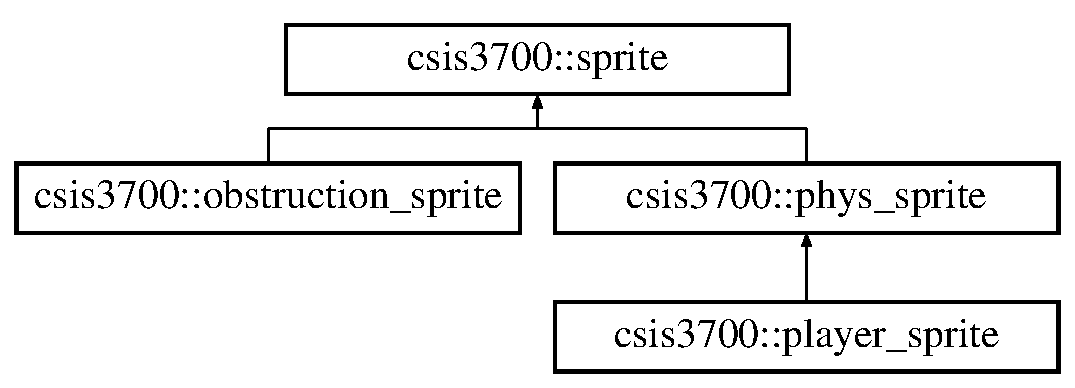
\includegraphics[height=3.000000cm]{classcsis3700_1_1sprite}
\end{center}
\end{figure}
\subsection*{Public Member Functions}
\begin{DoxyCompactItemize}
\item 
\hypertarget{classcsis3700_1_1sprite_a5395ad1b481e56895f11d57c7a052353}{{\bfseries sprite} (float initial\-\_\-x, float initial\-\_\-y)}\label{classcsis3700_1_1sprite_a5395ad1b481e56895f11d57c7a052353}

\item 
\hypertarget{classcsis3700_1_1sprite_a0b6e3ec9733f1300aac47ecf8570ee0b}{void {\bfseries set\-\_\-image\-\_\-sequence} (\hyperlink{classcsis3700_1_1image__sequence}{image\-\_\-sequence} $\ast$s)}\label{classcsis3700_1_1sprite_a0b6e3ec9733f1300aac47ecf8570ee0b}

\item 
virtual \hyperlink{classcsis3700_1_1sprite_a8f6db48ecf33279af2d084a344baae8c}{$\sim$sprite} ()
\item 
\hyperlink{classcsis3700_1_1sprite_adff79f206ea0703727a72287242fd8b1}{sprite} (const \hyperlink{classcsis3700_1_1sprite}{sprite} \&other)
\item 
\hypertarget{classcsis3700_1_1sprite_abd31e459d917f4789dd203730144e19a}{\hyperlink{classcsis3700_1_1sprite}{sprite} \& {\bfseries operator=} (const \hyperlink{classcsis3700_1_1sprite}{sprite} \&other)}\label{classcsis3700_1_1sprite_abd31e459d917f4789dd203730144e19a}

\item 
\hypertarget{classcsis3700_1_1sprite_a3ce0e3e67fc21797193f799b3c529630}{virtual int {\bfseries get\-\_\-width} () const }\label{classcsis3700_1_1sprite_a3ce0e3e67fc21797193f799b3c529630}

\item 
\hypertarget{classcsis3700_1_1sprite_a9f8719b41f7edeee77a56b548a339001}{virtual int {\bfseries get\-\_\-height} () const }\label{classcsis3700_1_1sprite_a9f8719b41f7edeee77a56b548a339001}

\item 
\hypertarget{classcsis3700_1_1sprite_af46c020f2e3c6e53c4d31300e7e3c9dc}{virtual float {\bfseries get\-\_\-x} () const }\label{classcsis3700_1_1sprite_af46c020f2e3c6e53c4d31300e7e3c9dc}

\item 
\hypertarget{classcsis3700_1_1sprite_aa546c86a477ef21fda91618d9e751bd8}{virtual float {\bfseries get\-\_\-y} () const }\label{classcsis3700_1_1sprite_aa546c86a477ef21fda91618d9e751bd8}

\item 
\hypertarget{classcsis3700_1_1sprite_acc128701e9bc6949168ce99ac7f95e70}{virtual \hyperlink{classcsis3700_1_1vec2d}{vec2d} {\bfseries get\-\_\-position} () const }\label{classcsis3700_1_1sprite_acc128701e9bc6949168ce99ac7f95e70}

\item 
\hypertarget{classcsis3700_1_1sprite_a433b1dbe4695990e42490d12d1bfac68}{virtual void {\bfseries set\-\_\-position} (\hyperlink{classcsis3700_1_1vec2d}{vec2d} p)}\label{classcsis3700_1_1sprite_a433b1dbe4695990e42490d12d1bfac68}

\item 
\hypertarget{classcsis3700_1_1sprite_a947c4b01559cbcd9c4dffbc6b39c6fbf}{virtual \hyperlink{classcsis3700_1_1vec2d}{vec2d} {\bfseries get\-\_\-velocity} () const =0}\label{classcsis3700_1_1sprite_a947c4b01559cbcd9c4dffbc6b39c6fbf}

\item 
\hypertarget{classcsis3700_1_1sprite_a3c43d72d94f5428d06d6f01b8753abe9}{virtual void {\bfseries set\-\_\-velocity} (const \hyperlink{classcsis3700_1_1vec2d}{vec2d} \&v)=0}\label{classcsis3700_1_1sprite_a3c43d72d94f5428d06d6f01b8753abe9}

\item 
\hypertarget{classcsis3700_1_1sprite_a01f24c59febf0c1fdd9ec0540ac02959}{virtual bool {\bfseries is\-\_\-passive} () const }\label{classcsis3700_1_1sprite_a01f24c59febf0c1fdd9ec0540ac02959}

\item 
virtual void \hyperlink{classcsis3700_1_1sprite_a6a69657522664635f116e05648792555}{draw} ()
\item 
virtual bool \hyperlink{classcsis3700_1_1sprite_a77871f0f7f7fca2af4b09302e9ec074c}{collides\-\_\-with} (const \hyperlink{classcsis3700_1_1sprite}{sprite} \&other) const 
\item 
virtual void \hyperlink{classcsis3700_1_1sprite_ac4d932bda87ce98a36579de3e1392a8f}{advance\-\_\-by\-\_\-time} (double dt)
\item 
virtual \hyperlink{classcsis3700_1_1rectangle}{rectangle} \hyperlink{classcsis3700_1_1sprite_a103e85a7cbc300db9c0f6bd5abb392dc}{bounding\-\_\-box} () const 
\item 
virtual \hyperlink{classcsis3700_1_1rectangle}{rectangle} \hyperlink{classcsis3700_1_1sprite_a979bf4a0de675c375146d4e6bc7365be}{collision\-\_\-rectangle} (const \hyperlink{classcsis3700_1_1sprite}{sprite} \&other) const 
\item 
\hypertarget{classcsis3700_1_1sprite_a4bf20253e1bc1825bfe73cdfcbb532d2}{virtual void {\bfseries resolve} (const \hyperlink{classcsis3700_1_1collision}{collision} \&\hyperlink{classcsis3700_1_1collision}{collision}, \hyperlink{classcsis3700_1_1sprite}{sprite} $\ast$other)=0}\label{classcsis3700_1_1sprite_a4bf20253e1bc1825bfe73cdfcbb532d2}

\end{DoxyCompactItemize}
\subsection*{Protected Attributes}
\begin{DoxyCompactItemize}
\item 
\hyperlink{classcsis3700_1_1vec2d}{vec2d} \hyperlink{classcsis3700_1_1sprite_aab9ac03c13c18eca432f5db06a8383b8}{position}
\item 
\hyperlink{classcsis3700_1_1image__sequence}{image\-\_\-sequence} $\ast$ \hyperlink{classcsis3700_1_1sprite_aa65b73f9bf7d266e57236f5b606b36e1}{sequence}
\item 
double \hyperlink{classcsis3700_1_1sprite_af12d2211006b3a184af6b70ed9e4235a}{time}
\end{DoxyCompactItemize}


\subsection{Constructor \& Destructor Documentation}
\hypertarget{classcsis3700_1_1sprite_a8f6db48ecf33279af2d084a344baae8c}{\index{csis3700\-::sprite@{csis3700\-::sprite}!$\sim$sprite@{$\sim$sprite}}
\index{$\sim$sprite@{$\sim$sprite}!csis3700::sprite@{csis3700\-::sprite}}
\subsubsection[{$\sim$sprite}]{\setlength{\rightskip}{0pt plus 5cm}csis3700\-::sprite\-::$\sim$sprite (
\begin{DoxyParamCaption}
{}
\end{DoxyParamCaption}
)\hspace{0.3cm}{\ttfamily [virtual]}}}\label{classcsis3700_1_1sprite_a8f6db48ecf33279af2d084a344baae8c}
Destructor \hypertarget{classcsis3700_1_1sprite_adff79f206ea0703727a72287242fd8b1}{\index{csis3700\-::sprite@{csis3700\-::sprite}!sprite@{sprite}}
\index{sprite@{sprite}!csis3700::sprite@{csis3700\-::sprite}}
\subsubsection[{sprite}]{\setlength{\rightskip}{0pt plus 5cm}csis3700\-::sprite\-::sprite (
\begin{DoxyParamCaption}
\item[{const {\bf sprite} \&}]{other}
\end{DoxyParamCaption}
)\hspace{0.3cm}{\ttfamily [inline]}}}\label{classcsis3700_1_1sprite_adff79f206ea0703727a72287242fd8b1}
these two should cause errors, no copying! 

\subsection{Member Function Documentation}
\hypertarget{classcsis3700_1_1sprite_ac4d932bda87ce98a36579de3e1392a8f}{\index{csis3700\-::sprite@{csis3700\-::sprite}!advance\-\_\-by\-\_\-time@{advance\-\_\-by\-\_\-time}}
\index{advance\-\_\-by\-\_\-time@{advance\-\_\-by\-\_\-time}!csis3700::sprite@{csis3700\-::sprite}}
\subsubsection[{advance\-\_\-by\-\_\-time}]{\setlength{\rightskip}{0pt plus 5cm}void csis3700\-::sprite\-::advance\-\_\-by\-\_\-time (
\begin{DoxyParamCaption}
\item[{double}]{dt}
\end{DoxyParamCaption}
)\hspace{0.3cm}{\ttfamily [virtual]}}}\label{classcsis3700_1_1sprite_ac4d932bda87ce98a36579de3e1392a8f}
Move time forward by the specified amount 

Reimplemented in \hyperlink{classcsis3700_1_1phys__sprite_a3bb24599b1bc2fd13846826308914db4}{csis3700\-::phys\-\_\-sprite}, and \hyperlink{classcsis3700_1_1player__sprite_ac2453e0b3934ac639d704c4ecca7493d}{csis3700\-::player\-\_\-sprite}.

\hypertarget{classcsis3700_1_1sprite_a103e85a7cbc300db9c0f6bd5abb392dc}{\index{csis3700\-::sprite@{csis3700\-::sprite}!bounding\-\_\-box@{bounding\-\_\-box}}
\index{bounding\-\_\-box@{bounding\-\_\-box}!csis3700::sprite@{csis3700\-::sprite}}
\subsubsection[{bounding\-\_\-box}]{\setlength{\rightskip}{0pt plus 5cm}{\bf rectangle} csis3700\-::sprite\-::bounding\-\_\-box (
\begin{DoxyParamCaption}
{}
\end{DoxyParamCaption}
) const\hspace{0.3cm}{\ttfamily [virtual]}}}\label{classcsis3700_1_1sprite_a103e85a7cbc300db9c0f6bd5abb392dc}
Return this sprite's bounding box \hypertarget{classcsis3700_1_1sprite_a77871f0f7f7fca2af4b09302e9ec074c}{\index{csis3700\-::sprite@{csis3700\-::sprite}!collides\-\_\-with@{collides\-\_\-with}}
\index{collides\-\_\-with@{collides\-\_\-with}!csis3700::sprite@{csis3700\-::sprite}}
\subsubsection[{collides\-\_\-with}]{\setlength{\rightskip}{0pt plus 5cm}bool csis3700\-::sprite\-::collides\-\_\-with (
\begin{DoxyParamCaption}
\item[{const {\bf sprite} \&}]{other}
\end{DoxyParamCaption}
) const\hspace{0.3cm}{\ttfamily [virtual]}}}\label{classcsis3700_1_1sprite_a77871f0f7f7fca2af4b09302e9ec074c}
Returns true iff I collide with other. Default implementation returns true iff my bounding box overlaps other's. \hypertarget{classcsis3700_1_1sprite_a979bf4a0de675c375146d4e6bc7365be}{\index{csis3700\-::sprite@{csis3700\-::sprite}!collision\-\_\-rectangle@{collision\-\_\-rectangle}}
\index{collision\-\_\-rectangle@{collision\-\_\-rectangle}!csis3700::sprite@{csis3700\-::sprite}}
\subsubsection[{collision\-\_\-rectangle}]{\setlength{\rightskip}{0pt plus 5cm}{\bf rectangle} csis3700\-::sprite\-::collision\-\_\-rectangle (
\begin{DoxyParamCaption}
\item[{const {\bf sprite} \&}]{other}
\end{DoxyParamCaption}
) const\hspace{0.3cm}{\ttfamily [virtual]}}}\label{classcsis3700_1_1sprite_a979bf4a0de675c375146d4e6bc7365be}
Return the intersection of this sprite's bounding box with other's bounding box. \hypertarget{classcsis3700_1_1sprite_a6a69657522664635f116e05648792555}{\index{csis3700\-::sprite@{csis3700\-::sprite}!draw@{draw}}
\index{draw@{draw}!csis3700::sprite@{csis3700\-::sprite}}
\subsubsection[{draw}]{\setlength{\rightskip}{0pt plus 5cm}void csis3700\-::sprite\-::draw (
\begin{DoxyParamCaption}
{}
\end{DoxyParamCaption}
)\hspace{0.3cm}{\ttfamily [virtual]}}}\label{classcsis3700_1_1sprite_a6a69657522664635f116e05648792555}
Draw this sprite. 

\subsection{Member Data Documentation}
\hypertarget{classcsis3700_1_1sprite_aab9ac03c13c18eca432f5db06a8383b8}{\index{csis3700\-::sprite@{csis3700\-::sprite}!position@{position}}
\index{position@{position}!csis3700::sprite@{csis3700\-::sprite}}
\subsubsection[{position}]{\setlength{\rightskip}{0pt plus 5cm}{\bf vec2d} csis3700\-::sprite\-::position\hspace{0.3cm}{\ttfamily [protected]}}}\label{classcsis3700_1_1sprite_aab9ac03c13c18eca432f5db06a8383b8}
My position \hypertarget{classcsis3700_1_1sprite_aa65b73f9bf7d266e57236f5b606b36e1}{\index{csis3700\-::sprite@{csis3700\-::sprite}!sequence@{sequence}}
\index{sequence@{sequence}!csis3700::sprite@{csis3700\-::sprite}}
\subsubsection[{sequence}]{\setlength{\rightskip}{0pt plus 5cm}{\bf image\-\_\-sequence}$\ast$ csis3700\-::sprite\-::sequence\hspace{0.3cm}{\ttfamily [protected]}}}\label{classcsis3700_1_1sprite_aa65b73f9bf7d266e57236f5b606b36e1}
My current image sequence \hypertarget{classcsis3700_1_1sprite_af12d2211006b3a184af6b70ed9e4235a}{\index{csis3700\-::sprite@{csis3700\-::sprite}!time@{time}}
\index{time@{time}!csis3700::sprite@{csis3700\-::sprite}}
\subsubsection[{time}]{\setlength{\rightskip}{0pt plus 5cm}double csis3700\-::sprite\-::time\hspace{0.3cm}{\ttfamily [protected]}}}\label{classcsis3700_1_1sprite_af12d2211006b3a184af6b70ed9e4235a}
The time in seconds since the world began ticking 

The documentation for this class was generated from the following files\-:\begin{DoxyCompactItemize}
\item 
sprite.\-h\item 
sprite.\-C\end{DoxyCompactItemize}

\hypertarget{classcsis3700_1_1vec2d}{\section{csis3700\-:\-:vec2d Class Reference}
\label{classcsis3700_1_1vec2d}\index{csis3700\-::vec2d@{csis3700\-::vec2d}}
}


{\ttfamily \#include $<$vec2d.\-h$>$}

\subsection*{Public Member Functions}
\begin{DoxyCompactItemize}
\item 
\hypertarget{classcsis3700_1_1vec2d_a40ee61b39f4e735dc12bd6030036c276}{{\bfseries vec2d} (float initial\-\_\-x=0, float initial\-\_\-y=0)}\label{classcsis3700_1_1vec2d_a40ee61b39f4e735dc12bd6030036c276}

\item 
\hypertarget{classcsis3700_1_1vec2d_ad99d90c512540cb22df3a34b6c748390}{float {\bfseries get\-\_\-x} () const }\label{classcsis3700_1_1vec2d_ad99d90c512540cb22df3a34b6c748390}

\item 
\hypertarget{classcsis3700_1_1vec2d_a238c5e6574ffa9a040733fd870542ff9}{float {\bfseries get\-\_\-y} () const }\label{classcsis3700_1_1vec2d_a238c5e6574ffa9a040733fd870542ff9}

\item 
\hyperlink{classcsis3700_1_1vec2d}{vec2d} \hyperlink{classcsis3700_1_1vec2d_a67675c0b80feaae1bde4be1153e71afb}{operator+} (const \hyperlink{classcsis3700_1_1vec2d}{vec2d} \&other) const 
\item 
\hyperlink{classcsis3700_1_1vec2d}{vec2d} \hyperlink{classcsis3700_1_1vec2d_a82b66d3d0e33548a49edb086a83c51ee}{operator-\/} (const \hyperlink{classcsis3700_1_1vec2d}{vec2d} \&other) const 
\item 
bool \hyperlink{classcsis3700_1_1vec2d_a8646bbf0141b775f1ff879ddc88f7032}{operator==} (const \hyperlink{classcsis3700_1_1vec2d}{vec2d} \&other) const 
\item 
\hyperlink{classcsis3700_1_1vec2d}{vec2d} \hyperlink{classcsis3700_1_1vec2d_a96895ad421dc29e595002a38cbd9db63}{max} (const \hyperlink{classcsis3700_1_1vec2d}{vec2d} \&other) const 
\item 
\hyperlink{classcsis3700_1_1vec2d}{vec2d} \hyperlink{classcsis3700_1_1vec2d_a88c04b0f27409ab448ded728b49ac976}{min} (const \hyperlink{classcsis3700_1_1vec2d}{vec2d} \&other) const 
\item 
\hyperlink{classcsis3700_1_1vec2d}{vec2d} \hyperlink{classcsis3700_1_1vec2d_ae79813cf256462512ddd3b293e074b05}{clamp} (float max\-\_\-x, float max\-\_\-y) const 
\item 
\hypertarget{classcsis3700_1_1vec2d_a2dc8b8021ffeed353db058f4815c8c24}{\hyperlink{classcsis3700_1_1vec2d}{vec2d} \& {\bfseries operator+=} (const \hyperlink{classcsis3700_1_1vec2d}{vec2d} \&other)}\label{classcsis3700_1_1vec2d_a2dc8b8021ffeed353db058f4815c8c24}

\end{DoxyCompactItemize}


\subsection{Detailed Description}
A 2-\/dimensional vector. Also used for point-\/like operations in which case, as a point, this vector is interpreted as the point corresponding to its endpoint if it began at the origin (that is a point with coordinates (x,y)). 

\subsection{Member Function Documentation}
\hypertarget{classcsis3700_1_1vec2d_ae79813cf256462512ddd3b293e074b05}{\index{csis3700\-::vec2d@{csis3700\-::vec2d}!clamp@{clamp}}
\index{clamp@{clamp}!csis3700::vec2d@{csis3700\-::vec2d}}
\subsubsection[{clamp}]{\setlength{\rightskip}{0pt plus 5cm}{\bf vec2d} csis3700\-::vec2d\-::clamp (
\begin{DoxyParamCaption}
\item[{float}]{max\-\_\-x, }
\item[{float}]{max\-\_\-y}
\end{DoxyParamCaption}
) const}}\label{classcsis3700_1_1vec2d_ae79813cf256462512ddd3b293e074b05}
Return a vector whose x component is between -\/max\-\_\-x and max\-\_\-x and whose y component is between -\/max\-\_\-y and max\-\_\-y. If the condition on the component is already met, do nothing to it, otherwise set it to the max with the appropriate sign. \hypertarget{classcsis3700_1_1vec2d_a96895ad421dc29e595002a38cbd9db63}{\index{csis3700\-::vec2d@{csis3700\-::vec2d}!max@{max}}
\index{max@{max}!csis3700::vec2d@{csis3700\-::vec2d}}
\subsubsection[{max}]{\setlength{\rightskip}{0pt plus 5cm}{\bf vec2d} csis3700\-::vec2d\-::max (
\begin{DoxyParamCaption}
\item[{const {\bf vec2d} \&}]{other}
\end{DoxyParamCaption}
) const}}\label{classcsis3700_1_1vec2d_a96895ad421dc29e595002a38cbd9db63}
Return a vector whose x is the max of this.\-x and other.\-x and whose y is the max of this.\-y and other.\-y. \hypertarget{classcsis3700_1_1vec2d_a88c04b0f27409ab448ded728b49ac976}{\index{csis3700\-::vec2d@{csis3700\-::vec2d}!min@{min}}
\index{min@{min}!csis3700::vec2d@{csis3700\-::vec2d}}
\subsubsection[{min}]{\setlength{\rightskip}{0pt plus 5cm}{\bf vec2d} csis3700\-::vec2d\-::min (
\begin{DoxyParamCaption}
\item[{const {\bf vec2d} \&}]{other}
\end{DoxyParamCaption}
) const}}\label{classcsis3700_1_1vec2d_a88c04b0f27409ab448ded728b49ac976}
Return a vector whose x is the min of this.\-x and other.\-x and whose y is the min of this.\-y and other.\-y. \hypertarget{classcsis3700_1_1vec2d_a67675c0b80feaae1bde4be1153e71afb}{\index{csis3700\-::vec2d@{csis3700\-::vec2d}!operator+@{operator+}}
\index{operator+@{operator+}!csis3700::vec2d@{csis3700\-::vec2d}}
\subsubsection[{operator+}]{\setlength{\rightskip}{0pt plus 5cm}{\bf vec2d} csis3700\-::vec2d\-::operator+ (
\begin{DoxyParamCaption}
\item[{const {\bf vec2d} \&}]{other}
\end{DoxyParamCaption}
) const}}\label{classcsis3700_1_1vec2d_a67675c0b80feaae1bde4be1153e71afb}
The vector sum of this and other. \hypertarget{classcsis3700_1_1vec2d_a82b66d3d0e33548a49edb086a83c51ee}{\index{csis3700\-::vec2d@{csis3700\-::vec2d}!operator-\/@{operator-\/}}
\index{operator-\/@{operator-\/}!csis3700::vec2d@{csis3700\-::vec2d}}
\subsubsection[{operator-\/}]{\setlength{\rightskip}{0pt plus 5cm}{\bf vec2d} csis3700\-::vec2d\-::operator-\/ (
\begin{DoxyParamCaption}
\item[{const {\bf vec2d} \&}]{other}
\end{DoxyParamCaption}
) const}}\label{classcsis3700_1_1vec2d_a82b66d3d0e33548a49edb086a83c51ee}
The vector difference (this -\/ other) \hypertarget{classcsis3700_1_1vec2d_a8646bbf0141b775f1ff879ddc88f7032}{\index{csis3700\-::vec2d@{csis3700\-::vec2d}!operator==@{operator==}}
\index{operator==@{operator==}!csis3700::vec2d@{csis3700\-::vec2d}}
\subsubsection[{operator==}]{\setlength{\rightskip}{0pt plus 5cm}bool csis3700\-::vec2d\-::operator== (
\begin{DoxyParamCaption}
\item[{const {\bf vec2d} \&}]{other}
\end{DoxyParamCaption}
) const}}\label{classcsis3700_1_1vec2d_a8646bbf0141b775f1ff879ddc88f7032}
Two vectors are equal iff their components are exactly equal. Be careful with floats! 

The documentation for this class was generated from the following files\-:\begin{DoxyCompactItemize}
\item 
vec2d.\-h\item 
vec2d.\-C\end{DoxyCompactItemize}

\hypertarget{classcsis3700_1_1world}{\section{csis3700\-:\-:world Class Reference}
\label{classcsis3700_1_1world}\index{csis3700\-::world@{csis3700\-::world}}
}
\subsection*{Public Member Functions}
\begin{DoxyCompactItemize}
\item 
\hyperlink{classcsis3700_1_1world_add94e82a5e7c88d9f4f2714c199693b1}{world} ()
\item 
\hyperlink{classcsis3700_1_1world_ae793effd77990768c2f7565cb2daba70}{$\sim$world} ()
\item 
\hyperlink{classcsis3700_1_1world_a323fcd5b15ee4a274bffe02cf9c7cd0e}{world} (const \hyperlink{classcsis3700_1_1world}{world} \&other)
\item 
\hyperlink{classcsis3700_1_1world}{world} \& \hyperlink{classcsis3700_1_1world_a1ce9a5a4c2a161b8d0bd079727632d62}{operator=} (const \hyperlink{classcsis3700_1_1world}{world} \&other)
\item 
void \hyperlink{classcsis3700_1_1world_a244cfed1968f6ed5133b82eebcb0c158}{handle\-\_\-event} (A\-L\-L\-E\-G\-R\-O\-\_\-\-E\-V\-E\-N\-T ev)
\item 
void \hyperlink{classcsis3700_1_1world_a2b4a33cc658001cde9d838ff50237a5f}{advance\-\_\-by\-\_\-time} (double dt)
\item 
void \hyperlink{classcsis3700_1_1world_acd1681a6ac117cf74ac4590938d60a80}{draw} ()
\end{DoxyCompactItemize}


\subsection{Constructor \& Destructor Documentation}
\hypertarget{classcsis3700_1_1world_add94e82a5e7c88d9f4f2714c199693b1}{\index{csis3700\-::world@{csis3700\-::world}!world@{world}}
\index{world@{world}!csis3700::world@{csis3700\-::world}}
\subsubsection[{world}]{\setlength{\rightskip}{0pt plus 5cm}csis3700\-::world\-::world (
\begin{DoxyParamCaption}
{}
\end{DoxyParamCaption}
)}}\label{classcsis3700_1_1world_add94e82a5e7c88d9f4f2714c199693b1}
Construct the world. The display is passed in simply to make it possible to modify options or access the backbuffer. D\-O N\-O\-T store the display in an instance variable. D\-O N\-O\-T start drawing on the screen. Just load bitmaps etc. \hypertarget{classcsis3700_1_1world_ae793effd77990768c2f7565cb2daba70}{\index{csis3700\-::world@{csis3700\-::world}!$\sim$world@{$\sim$world}}
\index{$\sim$world@{$\sim$world}!csis3700::world@{csis3700\-::world}}
\subsubsection[{$\sim$world}]{\setlength{\rightskip}{0pt plus 5cm}csis3700\-::world\-::$\sim$world (
\begin{DoxyParamCaption}
{}
\end{DoxyParamCaption}
)}}\label{classcsis3700_1_1world_ae793effd77990768c2f7565cb2daba70}
Free any resources being used by the world. \hypertarget{classcsis3700_1_1world_a323fcd5b15ee4a274bffe02cf9c7cd0e}{\index{csis3700\-::world@{csis3700\-::world}!world@{world}}
\index{world@{world}!csis3700::world@{csis3700\-::world}}
\subsubsection[{world}]{\setlength{\rightskip}{0pt plus 5cm}csis3700\-::world\-::world (
\begin{DoxyParamCaption}
\item[{const {\bf world} \&}]{other}
\end{DoxyParamCaption}
)}}\label{classcsis3700_1_1world_a323fcd5b15ee4a274bffe02cf9c7cd0e}
Block the copy constructor. Worlds should not be copied to just assert(false) 

\subsection{Member Function Documentation}
\hypertarget{classcsis3700_1_1world_a2b4a33cc658001cde9d838ff50237a5f}{\index{csis3700\-::world@{csis3700\-::world}!advance\-\_\-by\-\_\-time@{advance\-\_\-by\-\_\-time}}
\index{advance\-\_\-by\-\_\-time@{advance\-\_\-by\-\_\-time}!csis3700::world@{csis3700\-::world}}
\subsubsection[{advance\-\_\-by\-\_\-time}]{\setlength{\rightskip}{0pt plus 5cm}void csis3700\-::world\-::advance\-\_\-by\-\_\-time (
\begin{DoxyParamCaption}
\item[{double}]{dt}
\end{DoxyParamCaption}
)}}\label{classcsis3700_1_1world_a2b4a33cc658001cde9d838ff50237a5f}
Advance the state of the world forward by the specified time. \hypertarget{classcsis3700_1_1world_acd1681a6ac117cf74ac4590938d60a80}{\index{csis3700\-::world@{csis3700\-::world}!draw@{draw}}
\index{draw@{draw}!csis3700::world@{csis3700\-::world}}
\subsubsection[{draw}]{\setlength{\rightskip}{0pt plus 5cm}void csis3700\-::world\-::draw (
\begin{DoxyParamCaption}
{}
\end{DoxyParamCaption}
)}}\label{classcsis3700_1_1world_acd1681a6ac117cf74ac4590938d60a80}
Draw the world. Note that the display variable is passed only because it might be needed to switch the target bitmap back to the backbuffer. \hypertarget{classcsis3700_1_1world_a244cfed1968f6ed5133b82eebcb0c158}{\index{csis3700\-::world@{csis3700\-::world}!handle\-\_\-event@{handle\-\_\-event}}
\index{handle\-\_\-event@{handle\-\_\-event}!csis3700::world@{csis3700\-::world}}
\subsubsection[{handle\-\_\-event}]{\setlength{\rightskip}{0pt plus 5cm}void csis3700\-::world\-::handle\-\_\-event (
\begin{DoxyParamCaption}
\item[{A\-L\-L\-E\-G\-R\-O\-\_\-\-E\-V\-E\-N\-T}]{ev}
\end{DoxyParamCaption}
)}}\label{classcsis3700_1_1world_a244cfed1968f6ed5133b82eebcb0c158}
Update the state of the world based on the event ev. \hypertarget{classcsis3700_1_1world_a1ce9a5a4c2a161b8d0bd079727632d62}{\index{csis3700\-::world@{csis3700\-::world}!operator=@{operator=}}
\index{operator=@{operator=}!csis3700::world@{csis3700\-::world}}
\subsubsection[{operator=}]{\setlength{\rightskip}{0pt plus 5cm}{\bf world} \& csis3700\-::world\-::operator= (
\begin{DoxyParamCaption}
\item[{const {\bf world} \&}]{other}
\end{DoxyParamCaption}
)}}\label{classcsis3700_1_1world_a1ce9a5a4c2a161b8d0bd079727632d62}
Block operator =. Worlds should not be assigned. 

The documentation for this class was generated from the following files\-:\begin{DoxyCompactItemize}
\item 
world.\-h\item 
world.\-C\end{DoxyCompactItemize}

%--- End generated contents ---

% Index
\newpage
\phantomsection
\addcontentsline{toc}{chapter}{Index}
\printindex

\end{document}
